\documentclass{article}
\usepackage{fontspec}
\usepackage{xeCJK}
\usepackage{amsmath} % 数学公式支持
\usepackage{amsthm}  % 定理环境支持
\newtheorem{theorem}{Theorem}
\usepackage{graphicx}
\usepackage{tikz}
\usepackage{graphicx}
\usetikzlibrary{arrows.meta,3d}

% 中文字体设置
\setCJKmainfont{SimSun} % 宋体
\setCJKsansfont{SimHei} % 黑体
\setCJKmonofont{FangSong} % 仿宋

% 设置段落缩进和行距
\setlength{\parindent}{2em}
\setlength{\parskip}{1em}

\title{离散数学学期课程作业}
\author{离散数学第五小组}
\date{\today}

\begin{document}

\maketitle

\section{引言}


    在数学和计算机科学领域,等价关系作为一种满足自反性、对称性和传递性的二元关系,是将集合元素划分为等价类的理论基础。
等价关系的应用贯穿于众多领域,例如数论中的同余、逻辑中的等价公式以及图论中的节点划分等,
展现了其强大的问题简化能力。在计算机科学中,等价关系常被用来优化算法、压缩状态空间以及提升系统效率。

    本文以确定性有限自动机(Deterministic Finite Automaton, DFA)的状态最小化问题为切入点,
系统性地介绍等价关系的定义与性质,分析其在多个领域中的典型应用,并以 DFA 最小化为案例,
详细讲解如何利用等价关系划分状态集合,实现自动机的简化构造。通过理论与实践相结合,
本文旨在为读者提供理解等价关系及其应用的完整视角。

\newpage
\section{理论基础}
\subsection{等价关系的定义与性质}
    等价关系是一种二元关系$R$,若集合$A$上的二元关系$A$满足以下三个条件,称$\mathrm{R}$为等价关系:
\begin{enumerate}
    \item \textbf{自反性}: $\forall a \in A, (a,a) \in R$
    \item \textbf{对称性}: $\forall (a,b)\in R \rightarrow (b,a) \in R $
    \item \textbf{传递性}: $\forall a,b,c \in A, (a,b) \in R \wedge (b,c) \in R \rightarrow (a,c) \in R$
\end{enumerate}
\subsection{等价类与商集}
在等价关系 $\mathrm{R}$下,集合 $\mathrm{A}$可被划分为若干互不相交的等价类,
每个元素所属的等价类是其在 $\mathrm{R}$下的“等价群体”。
等价类的集合称为商集,记作$\mathrm{A}/\mathrm{R}$。这种划分为解决复杂问题提供了重要的结构化手段。

\subsection{应用意义}
等价关系通过将集合元素划分为等价类,减少了问题的复杂度。在许多算法中,等价关系作为划分与合并的理论基础,为优化问题提供了强有力的支持。


\newpage
\section{等价关系的应用}
\subsection{数学领域}
同余关系:模运算中,整数在模 $n$ 意义下形成的等价类,即同余类,是数论的基础工具之一。

\subsection{计算机科学领域}
状态最小化:DFA 最小化是等价关系在计算机科学中的经典应用之一,通过等价类划分实现状态压缩。
并查集:用于动态维护元素间等价关系的数据结构,广泛应用于图算法中,如最小生成树的构造。

\subsection{其他领域}
逻辑与推理:等价公式的判定与简化。
网络科学:在社交网络中分析等价节点的聚类特性。


\newpage
\section{等价关系在DFA中的应用}
\subsection{背景介绍}
    \textbf{DFA(deterministic finite automaton)}是一个有限状态机,通过接受由字符串唯一确定的状态序列来接受或拒绝给定的字符串
    \textbf{有限状态自动机}$M$是一个五元组$(Q, \Sigma, \delta, q_0, F)$,包含了
    \begin{itemize}
        \item 有限状态$Q$
        \item 有限输入符号$\Sigma$
        \item 转移函数$\delta: Q \times \Sigma \mapsto Q$
        \item 初识状态$q_0$
        \item 可接受状态集合$F \subset Q$
    \end{itemize}
    当一个字符串$w = a_0a_1\cdots a_n$输入状态机中,称$w$是可接受的当且仅当状态机接受$w$后产生的序列$r_0, r_1, \cdots, r_n$满足:
    \begin{enumerate}
        \item $r_0 = q_0$
        \item $r_{k+1} = \delta(r_k, q_k+1), for k = 0, 1, \ldots, n-1$
        \item $r_n \in F$
    \end{enumerate}
    称所有可接受的字符串为有限状态机$M$的语言,记为$L(M)$。
    
    其中$\delta$通常用状态转移表和状态转移图表示, 下面以一个$M_1$为例子。\\
    \begin{figure}[h]
        \centering
        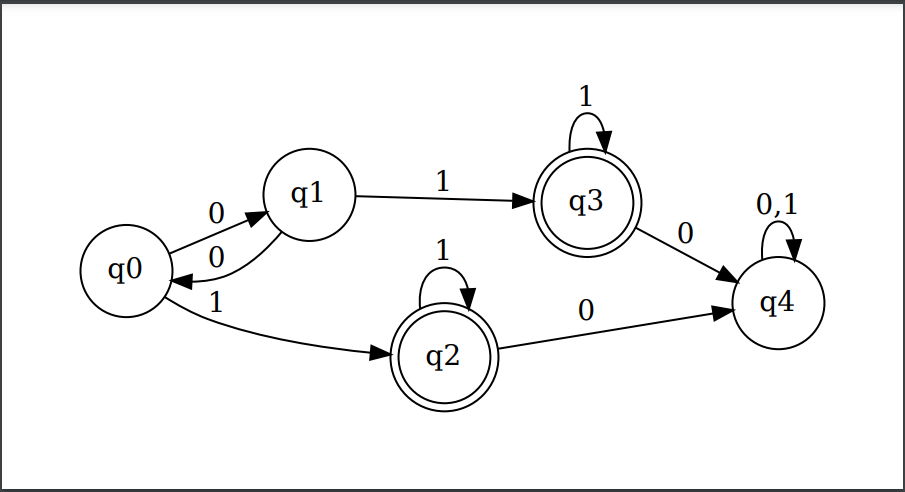
\includegraphics[scale=0.2]{../Img/dfa_example.png}
        \caption{有限状态机$M_1$的状态转移图}
    \end{figure}

    \begin{figure}[h]
        \centering
        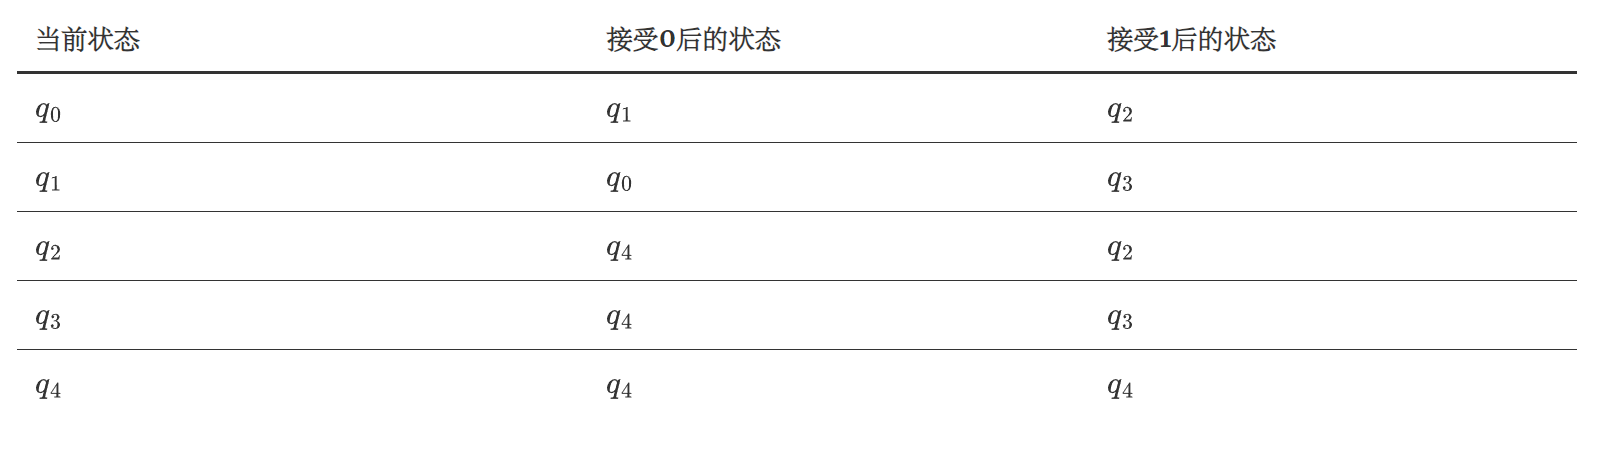
\includegraphics[scale=0.3]{../Img/minimized_pic.png}
    \end{figure}
    在有限状态机$M_1$中, $Q=\{q_0, q_1,q_2,q_3,q_4\}$, $\Sigma = \{0,1\}$, 初始状态为$q_0$
    可接受状态的集合$F = \{q_2, q_3\}$, 其中状态转移图由双圆圈标出的状态为可接受状态。


\subsection{等价关系在DFA中的应用}

在研究有穷自动机与正则表达式的关系时,一般引入等价关系对有穷自动机DFA的状态进行分类。对于任意一个自动机都可转换为
等价的确定有穷自动机\textbf{DFA},而确定有穷自动机 \textbf{DFA} 与正则集之间存在等价关系,即假定 $V=L(R)$,$R$ 是正则集 V 相对应的正则表达式。
$\Sigma$上的一个字集 $V \subset \Sigma^{*}$是正则的充分必要条件是存在 $\Sigma $上的确定有限自动机 \textbf{DFA} $M$使得:$V=L(M)$。 
对于任一给定的确定有穷自动机 \textbf{DFA} $M$,存在一个正则表达式 $R$,使得 $L(M)=L(R)$,反之亦然 。
下面以有穷自动机$M_2$为例进行演示。$M_2$的状态转移图如图2所示:
为了最小化 $M_2$,考虑状态$A$和$E$,先考虑接受以$0$开头的字符串:接受字符串$00$后,$A$转移至$G$状态,$E$转移至$G$状态;
接受字符串$01$后,$A$转移至$C$状态,$E$转移至$C$状态。由此可知,以$0$开头的字符串都可以将$A$,$E$带到同一个状态。

接着考虑以$1$开头的字符串:接受字符串$10$后$A$转移至$C$状态,$E$转移至$C$状态;接受字符串$11$后,$A$转移至$G$状态,
$E$转移至$G$状态。由此可知,以$1$开头的字符串都可以将$A,E$带到同一个状态


\begin{figure}[htbp]
    \centering
    \begin{minipage}{0.45\textwidth}
        \centering
        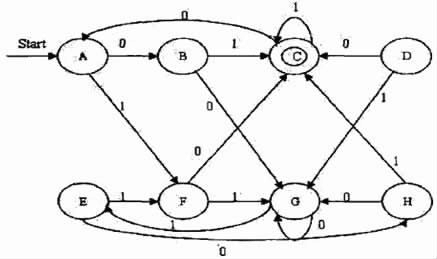
\includegraphics[width=\textwidth]{../Img/4_2_pic1.png}
        \caption{有限状态机M2的状态转移图}
    \end{minipage}
    \hfill
    \begin{minipage}{0.45\textwidth}
        \centering
        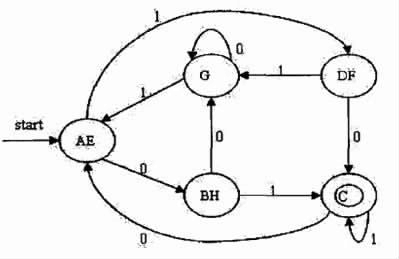
\includegraphics[width=\textwidth]{../Img/4_2_pic2.png}
        \caption{等价于M2的最小状态图}
    \end{minipage}
\end{figure}

以上的推演过程足以证明状态$A$和状态$E$是不可区分的,即状态$A$和状态$E$是等价的。
这样,据同样的算法来求出可区分状态对。最后,根据计算可知$(A,E),(H,B),(F,D)$具有等价关系。
最终形成一个等价类划分$[A,E][H,B][F,D][C][G]$。从而得到M2经过最小化的自动机如图 3 所示。



\subsection{DFA最小化意义}

由于在计算机科学和离散数学中,DFA是一种重要的数学模型,被广泛应用于正则语言的识别和处理。
DFA 最小化是一种通过减少状态数量来优化 DFA 的方法,它具有以下几个重要意义: 
\textbf{1. 减少资源消耗}

DFA 的状态数量直接影响其存储需求。每个状态在实现中通常会关联一组转移规则和可能的输出行为。
因此,状态数较多的 DFA 会占用更多的内存。通过最小化,等价的状态会被合并,从而降低了系统对
存储资源的需求。这在嵌入式系统或其他对资源高度敏感的环境中尤其重要。例如,在物联网设备中,
用于模式匹配的 DFA 最小化后可以减少存储需求,降低硬件成本。

\textbf{2. 提高运行效率}

在处理字符串时,DFA 的运行效率主要取决于状态的转换过程。最小化后的 DFA 减少了状态数量和冗余的转移路径
,这使得处理每个输入字符的时间更短。此外,较少的状态也意味着状态查找或状态表索引的开销降低,从而显著加
快运行速度。这种效率提升在实时处理系统中至关重要,例如语法解析器或网络数据包过滤中,都可以通过最小化后
的 DFA 保障系统的高效运行。

\textbf{3. 简化模型复杂性}

原始的 DFA 中可能存在许多等价状态和重复路径,这不仅增加了理解难度,还可能掩盖语言本质特征。通过
最小化,我们能够构造出结构最简单的 DFA,从而使自动机的核心逻辑更直观。

\textbf{4. 验证等价性}

两台 DFA 是否等价是一个重要的理论问题。由于最小化后的 DFA 是唯一的(即具有相同语言的最小化 DFA 在结构
上是相同的),它为验证等价性提供了简洁的手段。具体来说,可以通过将两个 DFA 分别最小化并比较其结果是否
一致来判断它们是否识别相同的语言。这种方法在编译器设计中尤其有用,例如确保优化后的正则表达式与原始版本
具有相同的功能。

\textbf{5. 提升可移植性和维护性}

DFA 的实际应用需要考虑跨系统的移植性。例如,在软件系统中,将 DFA 转换为硬件描述语言(如 Verilog)或嵌入式
代码时,最小化的 DFA 因其结构简洁,能大幅减少实现的复杂度。此外,由于最小化后的 DFA 不含冗余状态,其维护
成本显著降低:开发者可以更轻松地分析、扩展或修复逻辑问题。例如,在防火墙规则匹配系统中,最小化 DFA 不仅提
升匹配效率,还降低了错误的可能性。

 总之,DFA 最小化不仅是一种数学优化技术,也是一种能显著提升自动机实际应用价值的重要方法。通过该技术,可以在
 理论和实践中实现资源的高效利用,为各种计算和分析任务提供强有力的支持。



\subsection{DFA最小化方法}
    状态最小化一般分为两个步骤:
    \textbf{步骤一}
    首先,将 DFA 的所有状态分成两组:
    \begin{itemize}
        \item 结束状态(接受信号并输出结果的状态)。
        \item 非结束状态(不会输出结果的状态)。 
    \end{itemize}
    这两组不可能是相同的,因为它们在 DFA 中执行的功能显然不同。   

    \textbf{步骤二}
    然后,重复涉及 DFA 的所有状态,根据它们在接收信号后的转移情况进一步分组。举一个简单的示例:
    \begin{itemize}
        \item 如果状态 A 和 B 在接收同样的信号后,转向了同一组的其他状态,那么 A 和 B 可以视为相同状态,将它们合并。
        \item 如果不同,则它们需要分在不同组中。
    \end{itemize}
    这个过程是通过一种迭代方式完成的,直到没有更多的状态需要分组。

    \textbf{步骤三}
    最后,根据分组结果,将同一组的状态合并为一个新状态,构造出一个最小化后的 DFA。
    

下面将\textbf{4.3}中的有限状态机$M_1$进行化简:
首先将$DFA$中的状态$Q$分为结束状态/可接受状态$\{q_2,q_3\}$和非结束状态$\{q_0,q_1,q_4\}$
然后,将各组中所有状态根据接受不同字符后的结果进行分组,如果两个状态接受字符后结果相同(在同一分组中),则将这两个
状态分在一组,如果两个状态接受字符后结果不相同(比如一个在可接受状态,一个在非结束状态),则将这两个状态分入不同的
组中。

根据有限状态机的状态表可知,$q_2$和$q_3$接受$0$后的状态都是$q_4$,结果一致,$q_2$和$q_3$接受$1$后的结果分别是
$q_2$和$q_3$,都是本身,所以$q_2$和$q_3$接受$0,1$字符后结果一致,$\{q2,q_3\}$组保持不变

在$\{q_0,q_1,q_4\}$组中, $q_0$和$q_1$接受$0$后的结果分别是$q_1$和$q_0$,接受$1$后的结果分别是$q_2$,$q_3$,
而$q_2,q_3$是等价的,所以将$q_0$与$q_1$划入同一组,$q_0$与$q_4$接受$1$后的状态分别是$q_2$和$q_4$, 而$q_2$属于
可接受状态,$q_4$属于非结束状态,所以$q_0,q_1$与$q_4$不在同一组。

最终通过划分得到三个等价类$\{q_0,q_1\}$,$\{q_2,q_3\}$,$\{q_4\}$

根据原先的有限状态机的状态表重新绘制状态转移图,得到:

\begin{figure}[h]
    \centering
    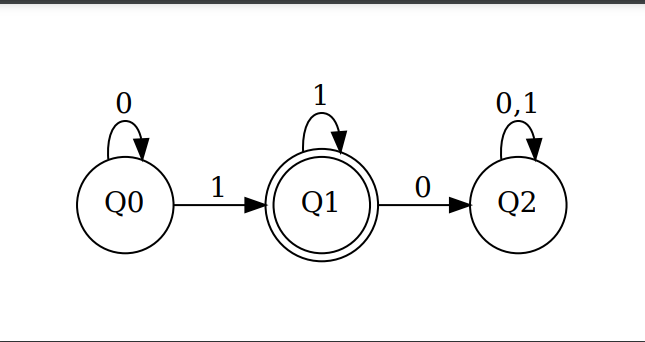
\includegraphics[scale=0.2]{../Img/minimized_dfa_example.png}
    \caption{化简后的状态转移图}
\end{figure}




\subsection{DFA最小化算法}
\subsubsection{Hopcraft算法}

\subsubsection{常翰堃算法(bushi)}
    这部分由常翰堃完成


\newpage
\section{总结}

在自动机理论中,DFA(确定性有限自动机)的最小化问题是一个核心研究课题,其研究不仅具有理论意义,也在
实际应用中展现出广泛价值。本文以等价类的定义与性质为基础,详细分析了 DFA 最小化的理论依据及其构造方
法,重点探讨了利用等价关系划分状态集合以实现自动机简化的具体步骤和应用价值。 等价类的概念在 DFA 最小
化中起到了理论支柱的作用。通过定义状态间的等价关系,我们能够将自动机的所有状态划分为若干等价类,每个
等价类代表一组功能完全相同的状态。DFA 最小化的核心在于通过状态等价的判 定,合并等价状态,构造具有最
少状态数的等价自动机。
   
   本文从理论层面阐述了最小化的必要性,包括降低存储空间需求、提高运行效率以及简化模型复杂度。在方法层
   面,我们采用了一种系统化的两步流程:首先区分终态与非终态,接着通过递归划分精确判定状态等价性,从而
   完成自动机最小化。实验表明,这些方法具有良好的通用性和实用性。在实际操作中,等价关系的构造是 DFA 最
   小化的关键步骤。本文详细分析了如何通过递归划分的方法确定状态集合的等价性,具体包括初始划分(终态与非
   终态)以及基于输入字符集的细化过程。通过不断细化状态集合,最终获得了不可进一步划分的等价类集合。这一
   过程不仅反映了集合论思想的具体应用,也展现了算法设计中递归与迭代方法的结合。

   在构造最小化 DFA 的过程中,本文采用了等价类划分法,通过状态等价类的代表元构建新的状态集合,并重新定义
   状态转移函数,实现了状态重命名与转移规则的高效重构。这一方法确保最小化后的自动机在语义上与原始自动机完
   全等价,但结构更加简洁紧凑。等价类划分法为 DFA 最小化提供了一条逻辑严谨且操作明确的路径,同时最小化 DFA
   的唯一性进一步验证了该方法的正确性与有效性。借助这一技术,最小化 DFA 能在语言等价性验证中展现重要价值,
   例如在编译器优化、正则表达式处理以及网络协议分析等领域,均发挥了显著的实践意义。

综上所述,本文通过等价类划分、状态最小化与自动机简化的系统研究,展示了 DFA 最小化在理论与实践中的重要意义
。这一研究不仅为离散数学与计算机科学的深入学习奠定了坚实基础,也为工程应用中的高效模式识别与系统优化提供
了参考方案。


\newpage
\section{参考文献}
\begin{enumerate}
    \item Hopcroft, J.E.Motwani, R.Ullman, J.D.(2007). $Introduction to Automata Theory,$ \newline$Languages, and Computation.$
    \item Sipser.M.(2013). $Introduction to the Theory of Computation. Cengage Learning.$
\end{enumerate}


\end{document}
